\documentclass[10pt]{llncs}

% obsługa języka polskiego
\usepackage[polish]{babel}	% pakiet niezbędny do obsługi języka polskiego
\usepackage[utf8]{inputenc}	% kodowanie dokumentu
\usepackage[T1]{fontenc}	% system kodowania czcionek
\usepackage{polski}		% słownik łamania wyrazów języka polskiego
\usepackage{indentfirst}	% wcięcie w każdym akapicie (polski standard drukarski)
\frenchspacing			% francuskie zwyczaje typograficzne (używane w Polsce)
\usepackage[pdftex]{graphicx}

% kolory
\usepackage[table]{xcolor}

% zapobieganie uciekaniu obrazów na następne strony (metoda \FloatBarrier)
\usepackage[section,subsection,subsubsection]{extraplaceins}

% algorytmy pisane w pseudokodzie
\usepackage{algpseudocode}
\usepackage{algorithm}
\usepackage{amsmath}

% typ czcionki
\usepackage{times}

% numerowanie stron
\pagestyle{headings}

\begin{document}
	
\title{Segmentacja przez progowanie (algorytmem Otsu) i przez klasteryzację (algorytmem ML-EM)}
\author{Maciej Górnicki, Bartosz Stalewski, Rafał Wojdowski}
\institute{CPOO, Dokumentacja projektu}
\maketitle

\section{Temat projektu}

Projekt polegał na zaimplementowaniu dwóch algorytmów służących do segmentacji obrazów na obszary:
\begin{itemize}
	\item algorytmu Otsu, wykonującego segmentację przez progowanie,
	\item algorytmu ML-EM, wykonującego segmentację przez klasteryzację. 
\end{itemize}

\section{Idee algorytmów}

\subsection{Algorytm Otsu}

Segmentacja metodą Otsu, której nazwa pochodzi od jej twórcy Nobuyuki Otsu, stanowi przykład progowania globalnego, w którym znalezione wartości progów są optymalne pod względem minimalizacji wariancji wewnątrzklasowej lub maksymalizacji wariancji międzyklasowej. Metoda Otsu osiąga dobre rezultaty na przykład dla obrazów o histogramach bimodalnych, czyli takich, gdzie możliwa jest reprezentacja histogramu przez dwa zachodzące na siebie rozkłady normalne o różnych wartościach średnich.

\subsection{Algorytm ML-EM}

Segmentacja metodą ML-EM (ang. Maximum Likelihood Estimation Maximization) polega na iteracyjnym szacowaniu parametrów modelu mikstur Gaussa. W takim modelu każdy klaster jest reprezentowany jako rozkład normalny o pewnej wartości średniej i macierzy kowariancji. W przypadku niniejszego projektu przestrzenią przeszukiwań, w której osadzone są klastry, jest przestrzeń czterowymiarowa $(R-G, R-B, i, j)$, gdzie $R - G$ to różnica między składową $R$ oraz $G$ piksela, $R - B$ to --- analogicznie --- różnica między składową $R$ oraz $B$ piksela, $i$ numer wiersza piksela, $j$ numer kolumny piksela.

\section{Testy algorytmu Otsu}

\subsection{Test algorytmu Otsu --- wybór jednego progu przy histogramie z dwoma skupiskami}

\begin{figure}[!htb]
\minipage{0.32\textwidth}
  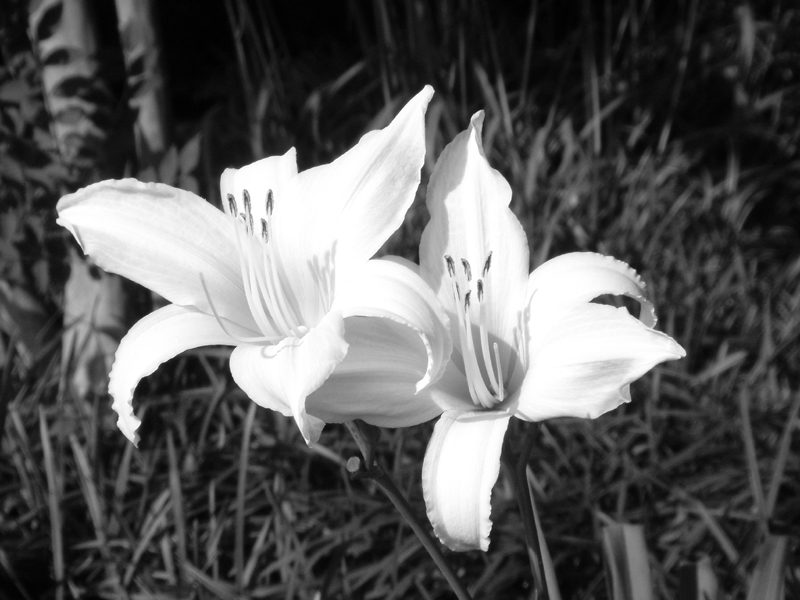
\includegraphics[width=\linewidth]{img/01.jpg}
  \caption{Rysunek wejściowy.}\label{fig:1}
\endminipage\hfill
\minipage{0.32\textwidth}
  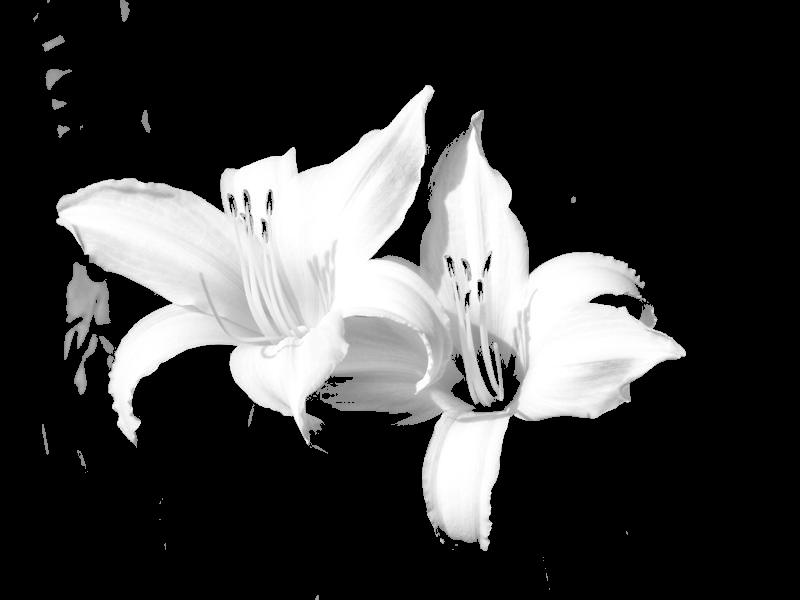
\includegraphics[width=\linewidth]{img/01_region_01.jpg}
  \caption{Region pierwszy (z dwóch) po segmentacji.}\label{fig:2}
\endminipage\hfill
\minipage{0.32\textwidth}
  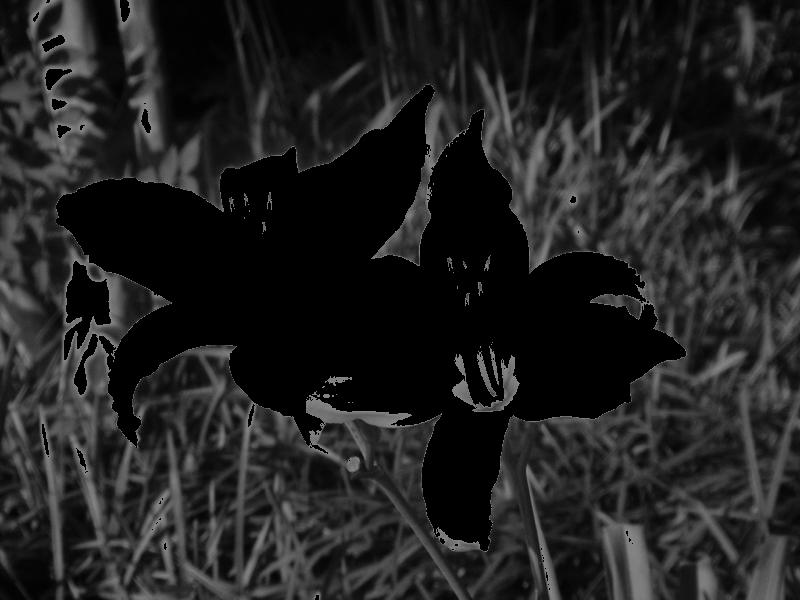
\includegraphics[width=\linewidth]{img/01_region_02.jpg}
  \caption{Region drugi (z dwóch) po segmentacji.}\label{fig:3}
\endminipage
\end{figure}

\begin{figure}[!htb]
\minipage{0.32\textwidth}
  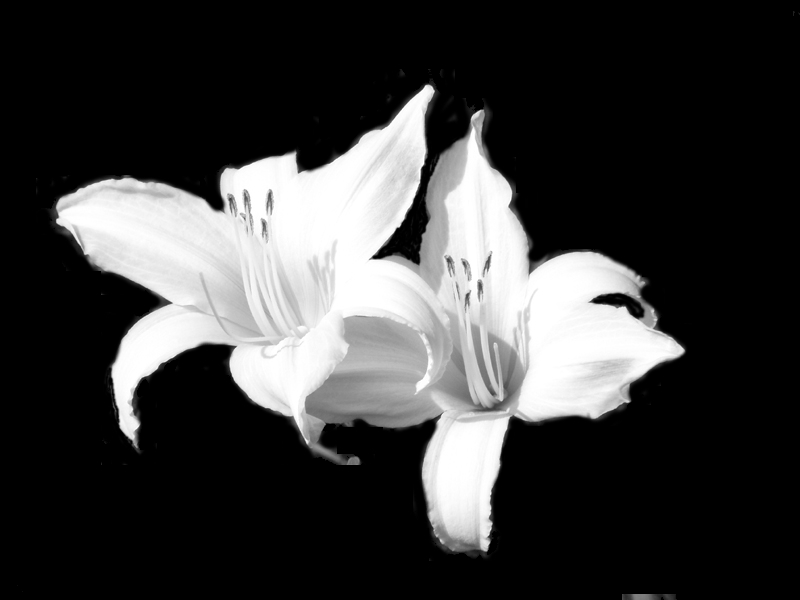
\includegraphics[width=\linewidth]{img/01_correct_segmentation.jpg}
  \caption{Region pierwszy (z dwóch) po segmentacji idealnej.}\label{fig:3_prim}
\endminipage\hfill
\end{figure}

\FloatBarrier

\begin{figure}[h!]
  \centering
  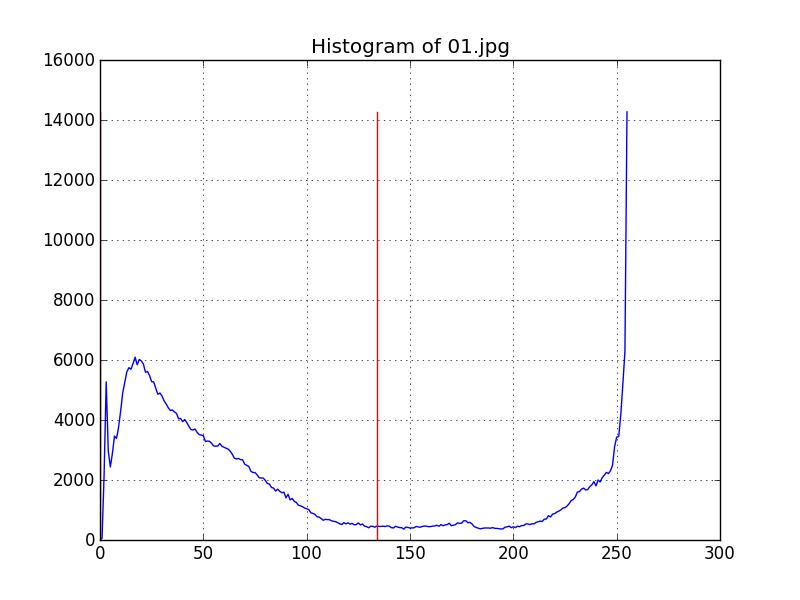
\includegraphics[scale=.3, clip]{img/01_histogram.jpg}
	\caption[]
  {Histogram rysunku wejściowego z zaznaczonym progiem, który został dobrany przez algorytm Otsu. Na podstawie histogramu da się zauważyć, że obraz wejściowy jest obrazem bimodalnym, czyli składającym się z pikseli, których jasności można zgrupować w dwóch skupiskach --- skupisku pikseli ciemnych (pikseli tła) i jasnych (pikseli pierwszego planu). Jak widać, próg (o wartości ok. 130) został dobrany dość dobrze, ponieważ znajduje się na środku pomiędzy oboma skupiskami.}
\end{figure}

\subsection{Test algorytmu Otsu --- wybór jednego progu przy histogramie z siedmioma skupiskami}

\begin{figure}[!htb]
\minipage{0.32\textwidth}
  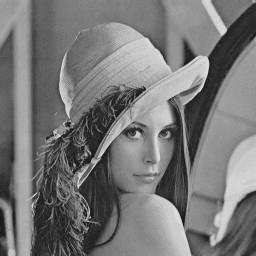
\includegraphics[width=\linewidth]{img/03.jpg}
  \caption{Rysunek wejściowy.}\label{fig:41}
\endminipage\hfill
\minipage{0.32\textwidth}
  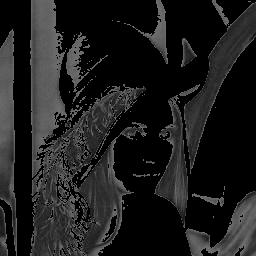
\includegraphics[width=\linewidth]{img/03_region_01.jpg}
  \caption{Region pierwszy (z dwóch) po segmentacji.}\label{fig:51}
\endminipage\hfill
\minipage{0.32\textwidth}
  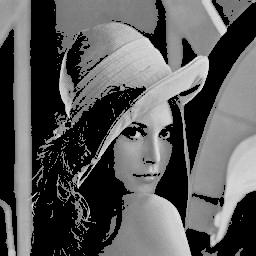
\includegraphics[width=\linewidth]{img/03_region_02.jpg}
  \caption{Region drugi (z dwóch) po segmentacji.}\label{fig:61}
\endminipage
\end{figure}

\begin{figure}[!htb]
\minipage{0.32\textwidth}
  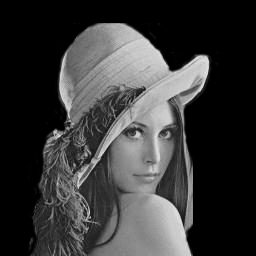
\includegraphics[width=\linewidth]{img/03_correct_segmentation.jpg}
  \caption{Region drugi (z dwóch) po segmentacji idealnej.}\label{fig:411}
\endminipage\hfill
\end{figure}

\begin{figure}[h!]
  \centering
  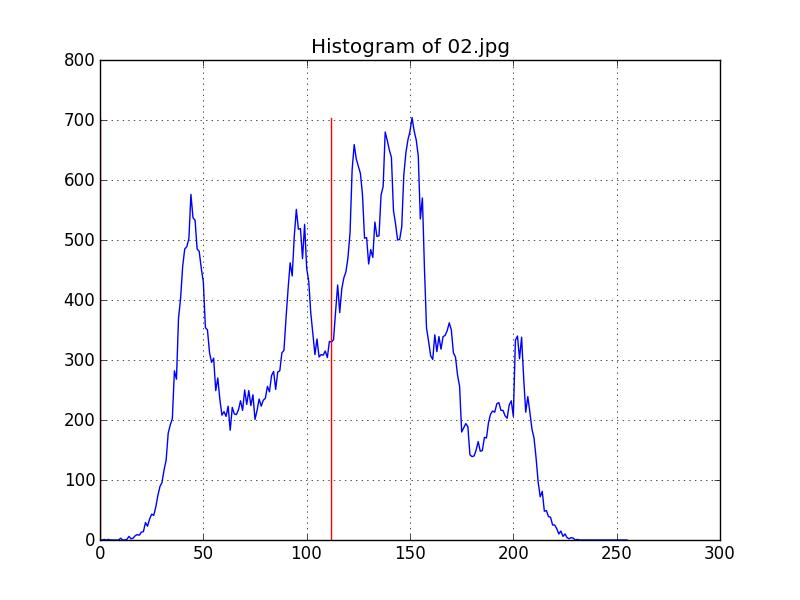
\includegraphics[scale=.3, clip]{img/03_histogram.jpg}
	\caption[]
  {Histogram rysunku wejściowego z zaznaczonym jednym progiem, który został dobrany przez algorytm Otsu. Jak widać, próg (o wartości ok. 120) został dobrany dość dobrze, ponieważ dzieli histogram na mniej więcej równe połowy pod względem ilości piseli znajdujących się po lewej i prawej stronie względem progu.}
\end{figure}

\subsection{Test algorytmu Otsu --- wybór czterech progów przy histogramie z siedmioma skupiskami}

\begin{figure}[!htb]
\minipage{0.32\textwidth}
  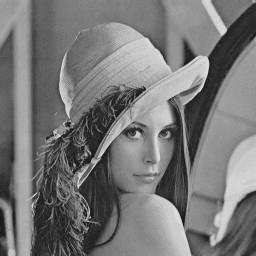
\includegraphics[width=\linewidth]{img/02.jpg}
  \caption{Rysunek wejściowy.}\label{fig:4}
\endminipage\hfill
\minipage{0.32\textwidth}
  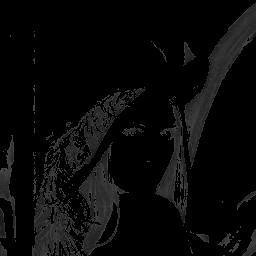
\includegraphics[width=\linewidth]{img/02_region_01.jpg}
  \caption{Region pierwszy (z pięciu) po segmentacji.}\label{fig:5}
\endminipage\hfill
\minipage{0.32\textwidth}
  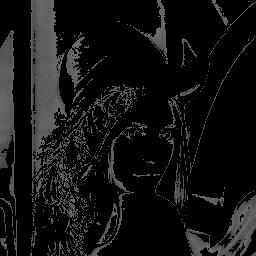
\includegraphics[width=\linewidth]{img/02_region_02.jpg}
  \caption{Region drugi (z pięciu) po segmentacji.}\label{fig:6}
\endminipage
\end{figure}

\begin{figure}[!htb]
\minipage{0.32\textwidth}
  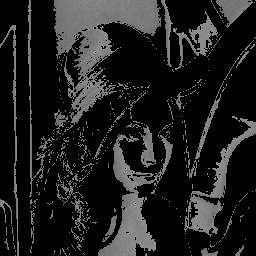
\includegraphics[width=\linewidth]{img/02_region_03.jpg}
  \caption{Region trzeci (z pięciu) po segmentacji.}\label{fig:7}
\endminipage\hfill
\minipage{0.32\textwidth}
  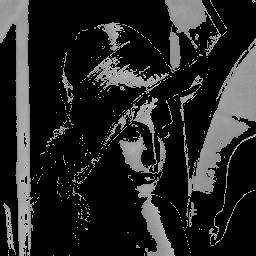
\includegraphics[width=\linewidth]{img/02_region_04.jpg}
  \caption{Region czwarty (z pięciu) po segmentacji.}\label{fig:8}
\endminipage\hfill
\minipage{0.32\textwidth}
  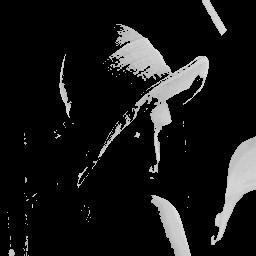
\includegraphics[width=\linewidth]{img/02_region_05.jpg}
  \caption{Region piąty (z pięciu) po segmentacji.}\label{fig:9}
\endminipage
\end{figure}

\begin{figure}[h!]
  \centering
  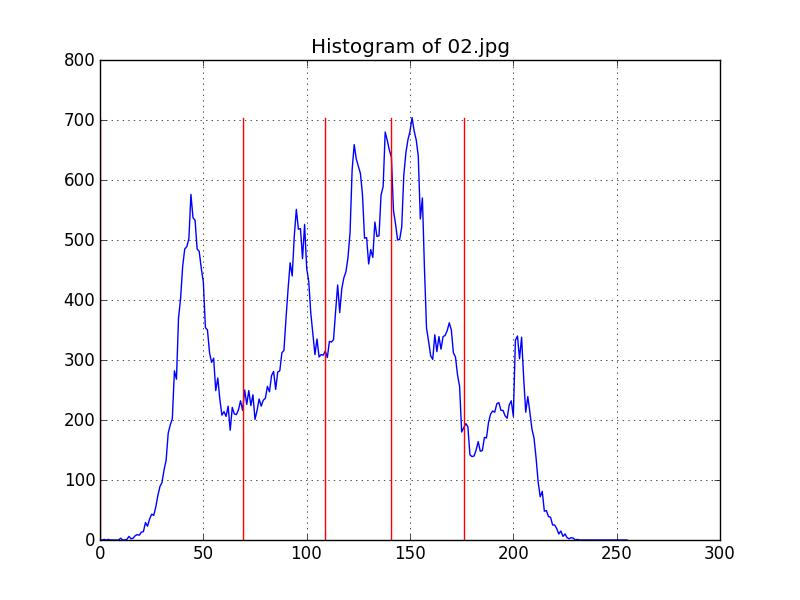
\includegraphics[scale=.3, clip]{img/02_histogram.jpg}
	\caption[]
  {Histogram rysunku wejściowego z zaznaczonymi czteroma progami, które zostały dobrane przez algorytm Otsu. Jak widać, progi zostały dobrane dość dobrze, ponieważ --- po pierwsze --- znajdują się mniej więcej na środku pomiędzy skupiskami i --- po drugie --- są od siebie oddalone w mniej więcej równych odstępach.}
\end{figure}

\subsection{Test algorytmu Otsu --- wybór jednego progu przy histogramie z jednym skupiskiem}

\begin{figure}[!htb]
\minipage{0.32\textwidth}
  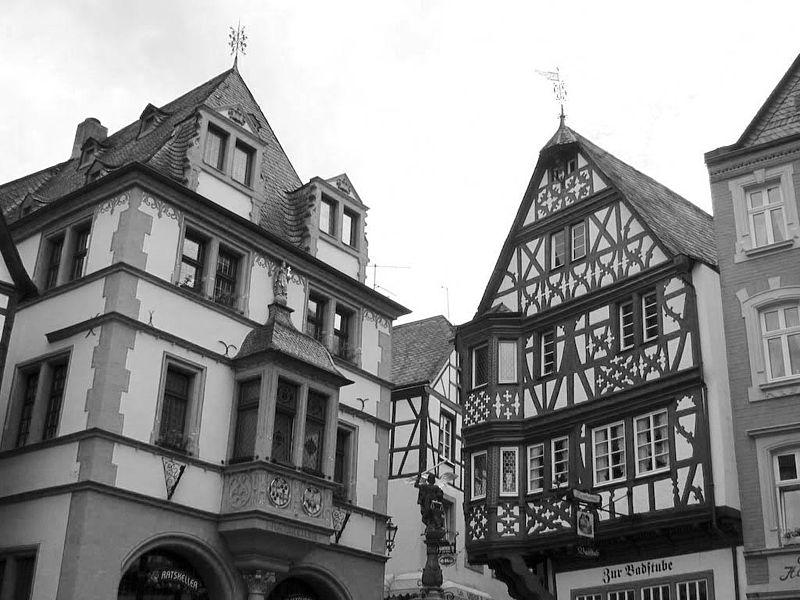
\includegraphics[width=\linewidth]{img/04.jpg}
  \caption{Rysunek wejściowy.}\label{fig:111}
\endminipage\hfill
\minipage{0.32\textwidth}
  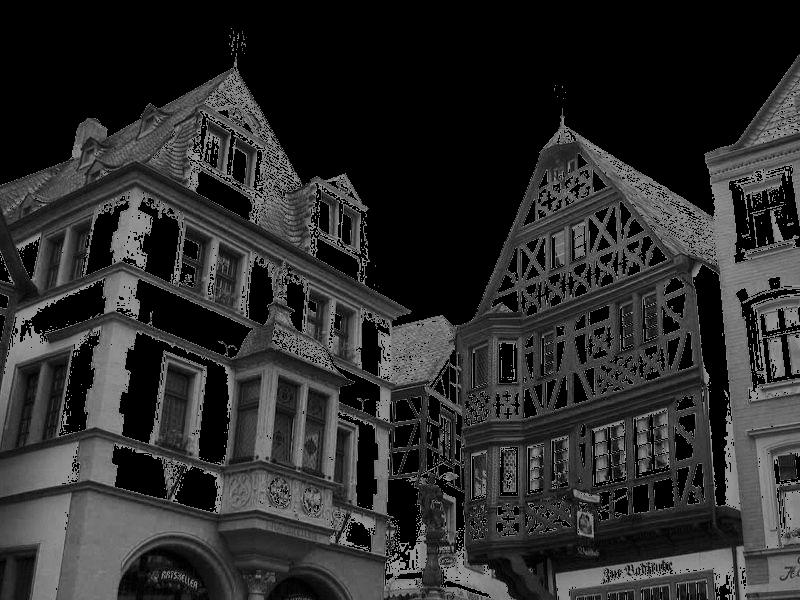
\includegraphics[width=\linewidth]{img/04_region_01.jpg}
  \caption{Region pierwszy (z dwóch) po segmentacji.}\label{fig:211}
\endminipage\hfill
\minipage{0.32\textwidth}
  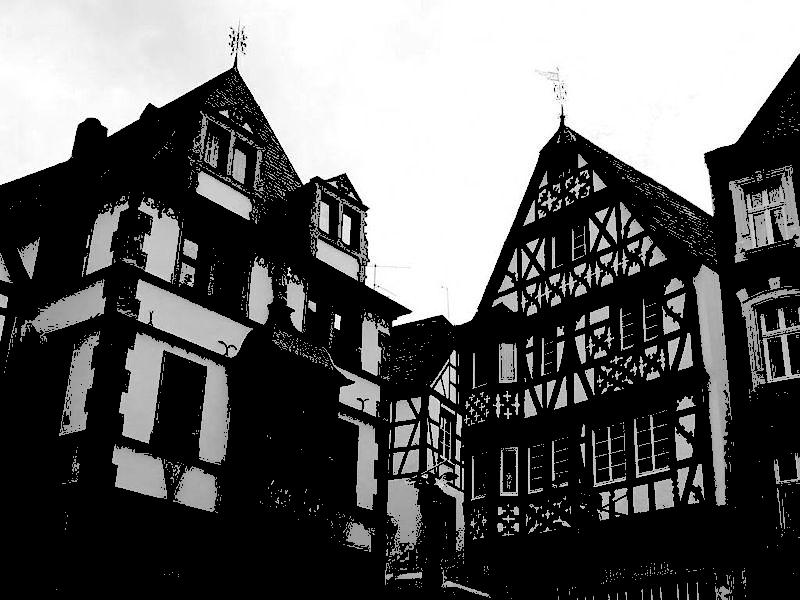
\includegraphics[width=\linewidth]{img/04_region_02.jpg}
  \caption{Region drugi (z dwóch) po segmentacji.}\label{fig:311}
\endminipage
\end{figure}

\begin{figure}[!htb]
\minipage{0.32\textwidth}
  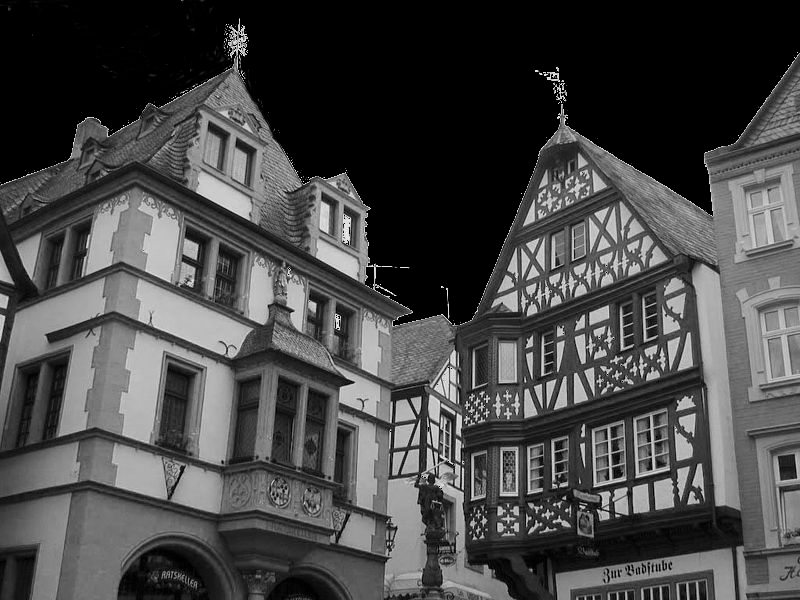
\includegraphics[width=\linewidth]{img/04_correct_segmentation.jpg}
  \caption{Region pierwszy (z dwóch) po segmentacji idealnej.}\label{fig:3_prim}
\endminipage\hfill
\end{figure}

\FloatBarrier

\begin{figure}[h!]
  \centering
  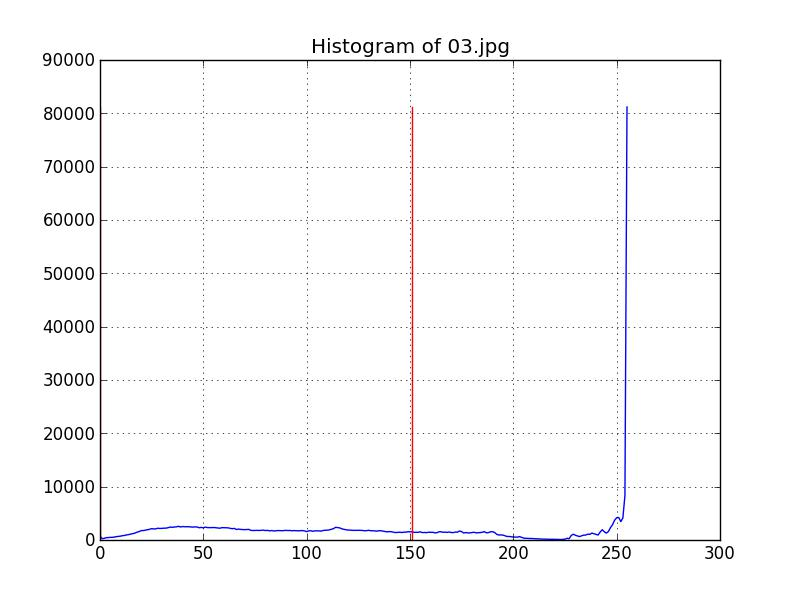
\includegraphics[scale=.3, clip]{img/04_histogram.jpg}
	\caption[]
  {Histogram rysunku wejściowego z zaznaczonym progiem, który został dobrany przez algorytm Otsu. Jak widać, próg (o wartości ok. 150) został dobrany dość dobrze, ponieważ oddziela piksele najciemniejsze od najjaśniejszych, nia nachodząc na największe skupisko pikseli.}
\end{figure}

\section{Testy algorytmu ML-EM}

\subsection{Test algorytmu ML-EM --- wybór pięciu obszarów}

\begin{figure}[!htb]
\minipage{0.32\textwidth}
  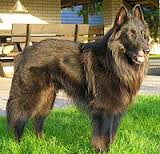
\includegraphics[width=\linewidth]{img/images.jpg}
  \caption{Rysunek wejściowy.}\label{fig:10}
\endminipage\hfill
\minipage{0.32\textwidth}
  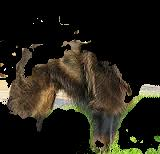
\includegraphics[width=\linewidth]{img/images_k5_0.jpg}
  \caption{Region pierwszy (z pięciu) po segmentacji.}\label{fig:11}
\endminipage\hfill
\minipage{0.32\textwidth}
  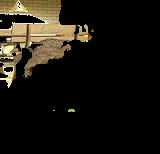
\includegraphics[width=\linewidth]{img/images_k5_1.jpg}
  \caption{Region drugi (z pięciu) po segmentacji.}\label{fig:12}
\endminipage
\end{figure}

\begin{figure}[!htb]
\minipage{0.32\textwidth}
  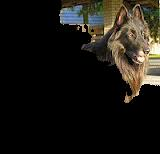
\includegraphics[width=\linewidth]{img/images_k5_2.jpg}
  \caption{Region trzeci (z pięciu) po segmentacji.}\label{fig:10}
\endminipage\hfill
\minipage{0.32\textwidth}
  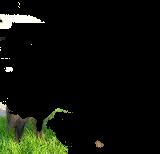
\includegraphics[width=\linewidth]{img/images_k5_3.jpg}
  \caption{Region czwarty (z pięciu) po segmentacji.}\label{fig:11}
\endminipage\hfill
\minipage{0.32\textwidth}
  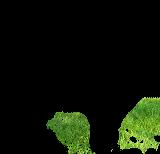
\includegraphics[width=\linewidth]{img/images_k5_4.jpg}
  \caption{Region piąty (z pięciu) po segmentacji.}\label{fig:12}
\endminipage
\end{figure}

\subsection{Test algorytmu ML-EM --- wybór dwóch obszarów}

\begin{figure}[!htb]
\minipage{0.32\textwidth}
  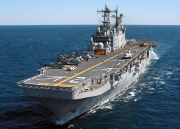
\includegraphics[width=\linewidth]{img/ship.jpg}
  \caption{Rysunek wejściowy.}\label{fig:13}
\endminipage\hfill
\minipage{0.32\textwidth}
  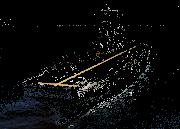
\includegraphics[width=\linewidth]{img/ship_k2_0.jpg}
  \caption{Region pierwszy (z dwóch) po segmentacji.}\label{fig:14}
\endminipage\hfill
\minipage{0.32\textwidth}
  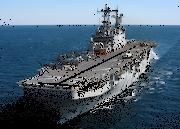
\includegraphics[width=\linewidth]{img/ship_k2_1.jpg}
  \caption{Region drugi (z dwóch) po segmentacji.}\label{fig:15}
\endminipage
\end{figure}

\subsection{Test algorytmu ML-EM --- wybór pięciu obszarów}

\begin{figure}[!htb]
\minipage{0.32\textwidth}
  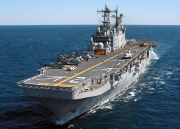
\includegraphics[width=\linewidth]{img/ship.jpg}
  \caption{Rysunek wejściowy.}\label{fig:16}
\endminipage\hfill
\minipage{0.32\textwidth}
  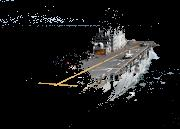
\includegraphics[width=\linewidth]{img/ship_k5_0.jpg}
  \caption{Region pierwszy (z pięciu) po segmentacji.}\label{fig:17}
\endminipage\hfill
\minipage{0.32\textwidth}
  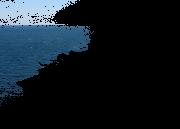
\includegraphics[width=\linewidth]{img/ship_k5_1.jpg}
  \caption{Region drugi (z pięciu) po segmentacji.}\label{fig:18}
\endminipage
\end{figure}

\begin{figure}[!htb]
\minipage{0.32\textwidth}
  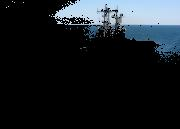
\includegraphics[width=\linewidth]{img/ship_k5_2.jpg}
  \caption{Region trzeci (z pięciu) po segmentacji.}\label{fig:19}
\endminipage\hfill
\minipage{0.32\textwidth}
  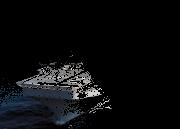
\includegraphics[width=\linewidth]{img/ship_k5_3.jpg}
  \caption{Region czwarty (z pięciu) po segmentacji.}\label{fig:20}
\endminipage\hfill
\minipage{0.32\textwidth}
  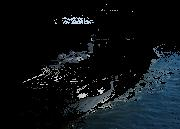
\includegraphics[width=\linewidth]{img/ship_k5_4.jpg}
  \caption{Region piąty (z pięciu) po segmentacji.}\label{fig:21}
\endminipage
\end{figure}

\FloatBarrier

\end{document}